\documentclass[]{article}
\usepackage{amsmath, amsfonts}
\usepackage{enumitem}
\usepackage{fancyhdr}
\usepackage{geometry}
\usepackage{cancel}
\usepackage{graphicx}
\usepackage{color}
\usepackage{soul}
\usepackage{multirow}
\usepackage{float}
\usepackage{pgfplots}	% To draw charts directly in Latex
\usepackage{marvosym}	% For lightning symbol to denote contradiction
\usepackage{cleveref}	% For clever referencing :)
\usepackage{nameref}	% For referencing to the section name, not number

%TikZ package for drawing:
\usepackage{tikz}
%For calculation of coordinates:
\usetikzlibrary{calc}
\usetikzlibrary{positioning}

%opening
\title{Exam 2015 - 2016\\ \large Microeconomics II}
\author{Nurfatima Jandarova}
\date{\today}
\pagestyle{fancy}

\lhead{Microeconomics II, Exam 2015 - 2016}
\rhead{Nurfatima Jandarova}
\renewcommand{\headrulewidth}{0.4pt}
\fancyheadoffset{1 cm}

\geometry{a4paper, left=20mm, top=20mm, bottom = 20mm, headheight=20mm}

\sloppy
\definecolor{lightgray}{gray}{0.5}
\setlength{\parindent}{0pt}

\renewcommand{\arraystretch}{1.3}

\setul{0.2ex}{0.2ex}
\setulcolor{red}

\begin{document}

\maketitle

\subsection*{Question 1}
\subsubsection*{1}
The game in extensive form:
\begin{figure}[h]
	\begin{center}
		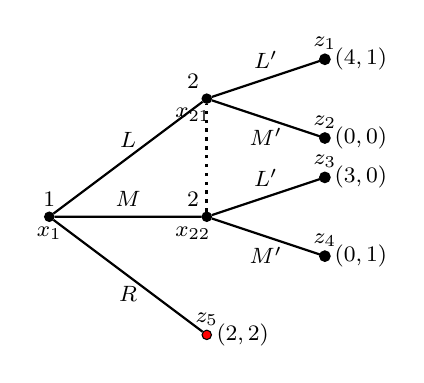
\begin{tikzpicture}
		[
		grow =right,
		font=\footnotesize,
		edge from parent/.style={draw,thick}
		]
		
		% Two node styles: solid and hollow
		\tikzstyle{solid node}=[circle,draw,inner sep=1.2,fill=black];
		\tikzstyle{end node}=[circle,draw,inner sep=1.2,fill=red];
		\tikzstyle{hollow node}=[circle,draw,inner sep=1.2];
		
		% Specify spacing for each level of the tree
		\tikzstyle{level 1}=[level distance=20mm,sibling distance=15mm]
		\tikzstyle{level 2}=[level distance=15mm,sibling distance=10mm]
		\tikzstyle{level 3}=[level distance=15mm,sibling distance=5mm]
		% The Tree
		\node(0)[solid node]{}
		% R
		child{node[end node]{} edge from parent node[below]{$R$}}
		% M
		child{node[solid node]{} 
			child{node[solid node]{} edge from parent node[below]{$M'$}}
			child{node[solid node]{} edge from parent node[above]{$L'$}}
		edge from parent node[above]{$M$}}
		% M
		child{node[solid node]{} 
			child{node[solid node]{} edge from parent node[below]{$M'$}}
			child{node[solid node]{} edge from parent node[above]{$L'$}}
		edge from parent node[above]{$L$}}
		;
		% Information sets
		\draw[dotted,very thick](0-2)to(0-3);
		
		% Players
		% player 1
		\node[above]at(0){1};
		% player 2
		\foreach \x in {2, 3} \node[above, xshift=-5]at(0-\x){2};
		
		% Specifying payoffs
		% Stop
		\node[right]at(0-1){$(2, 2)$};
		\node[right]at(0-2-1){$(0, 1)$};
		\node[right]at(0-2-2){$(3, 0)$};
		\node[right]at(0-3-1){$(0, 0)$};
		\node[right]at(0-3-2){$(4, 1)$};
		
		% Naming the nodes
		\node[below]at(0){$x_1$};
		\node[above]at(0-1){$z_5$};
		\node[below, xshift=-5]at(0-2){$x_{22}$};
		\node[below, xshift=-5]at(0-3){$x_{21}$};
		\node[above]at(0-3-2){$z_1$};
		\node[above]at(0-3-1){$z_2$};
		\node[above]at(0-2-2){$z_3$};
		\node[above]at(0-2-1){$z_4$};
		\end{tikzpicture}
	\end{center}
%	\caption{A centipede game in extensive form}
%	\label{fig:ex1ext}
\end{figure}

There are two players, i.e., $N = \{1, 2\}$. $K = \{x_1, x_{21},x_{22}, z_1, z_2, z_3, z_4, z_5\}$ and $P(x_1) = \emptyset$, $x_{21}Rz_1$, $x_{21}Rz_2$, $x_{22}Rz_3$, $x_{22}Rz_4$. The set of nodes is partitioned between the two players in the following way: $K_1 = \{x_1\}$ and $K_2 = \{x_{21}, x_{22}\}$. The information sets are defined as follows: $H_1 = K_1$ and $H_2 = K_2$.
The strategy spaces of the two players are: $S_1 = \{L, M, R\}$ and $S_2 = \{L', M'\}$. The profit functions are
\begin{equation}
	\begin{split}
		\pi_1: S_1\times S_2 \to \{0, 2, 3, 4\} \\ \nonumber
		\pi_2: S_2\times S_1 \to \{0, 1, 2\}
	\end{split}
\end{equation}
and could be tabulated as
\begin{table}[h]
	\centering
	\begin{tabular}{c|cc}
		 & L' & M' \\ \hline
		L & (\ul{4}, \ul{1}) & (0, 0) \\
		M & (3, 0) & (0, \ul{1}) \\
		R & (2, \ul{2}) & (\ul{2}, \ul{2})
	\end{tabular}
\end{table}

\subsubsection*{2}

To find Nash equilibria, need to find intersection of best responses of the two players. Those are underlined in the table above. Hence, there are two NE in pure strategies, $\{(L, L'), (R, M')\}$.

\begin{figure}[h]
	\centering
	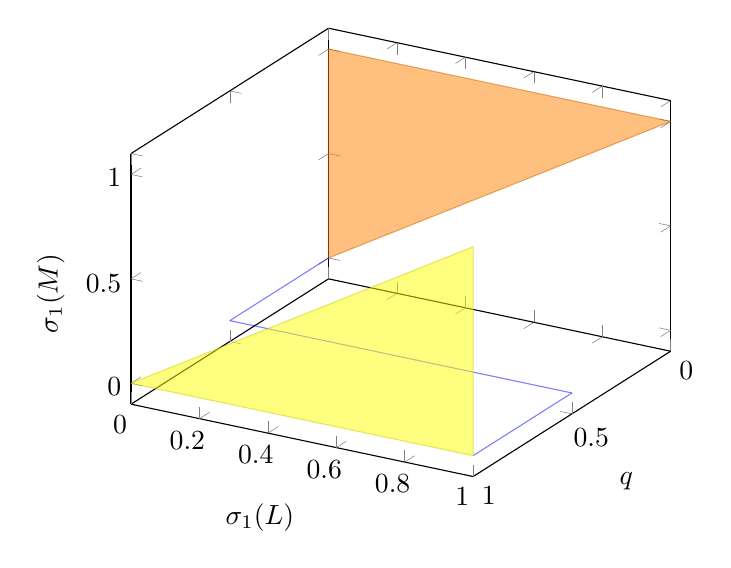
\begin{tikzpicture}
		\begin{axis}[
			view/h=120, 
			xlabel=$q$, ylabel=$\sigma_1(L)$, zlabel=$\sigma_1(M)$,
			ymajorgrids=false,
			]
			
			% Best response of player 1
			\addplot3[
			opacity = 0.5, 
			table/row sep = \\, 
			mesh,
			] 
			table {
			x y z\\
			0 0 0 \\
			0.5 0 0 \\
			0.5 1 0 \\
			1 1 0\\};
			
			% Best response of player 2
			\addplot3[
			opacity = 0.5, 
			table/row sep = \\, 
			patch,
			] 
			table {
				x y z\\
%				0 1 1 \\
				0 0 1 \\
				0 0 0 \\
				0 1 1 \\
				1 0 0 \\ 
				1 1 0 \\
				1 1 1 \\
%				1 0 0 \\
%				0 0 0 \\
%				1 1 1 \\
%				0 1 1 \\
				};
		\end{axis}
	\end{tikzpicture}
\end{figure}

Since there's only one proper subgame, the entire game itself, the set of NE in pure strategies is the same as the set of SGPE in pure strategies.

\subsubsection*{3}

Let $\mu$ denote the system of beliefs of player 2 in his information set, $\mu = (\mu(x_{21}, 1 - \mu(x_{21})))$.
\begin{equation}
	\begin{split}
		\begin{matrix}
			\text{Player 2 chooses }L'\text{ if} \\
			\mu(x_{21}) > 1 - \mu(x_{21}) \\
			\mu(x_{21}) > \frac{1}{2}
		\end{matrix} \qquad\qquad \begin{matrix}
			\text{Player 2 chooses }M'\text{ if} \\
			\mu(x_{21}) < 1 - \mu(x_{21}) \\
			\mu(x_{21}) < \frac{1}{2}
		\end{matrix} \nonumber
	\end{split}
\end{equation}

Suppose the belief system $\mu$ is such that $\mu(x_{21}) > \frac{1}{2}$, i.e., player 2 chooses $L'$. Then, by sequential rationality, player 1 chooses $L$. This implies a strategy $\gamma = (L, L')$. Given this strategy, $P^\gamma(H_2) = 1$ and $P^\gamma(x_{21}) = 1$. Thus, to be statistically consistent, $\mu(x_{21}) = \frac{P^\gamma(x_{21})}{P^\gamma(H_2)} = 1$, which also satisfies the initial condition on the belief system for player 2 to choose $L'$. Hence, a strategy $(L, L')$ and a belief system $\mu = (1, 0)$ constitute a WPBE.

Now, consider another case, where $\mu(x_{21}) < \frac{1}{2}$, i.e., player 2 chooses $M'$. Then, by sequential rationality, player 1 chooses $R$. This implies that the information set $H_2$ is never reached, and any belief system of player 2 is consistent. Therefore, a strategy $(R, M')$ and any belief system such that $\mu(x_{21}) < \frac{1}{2}$ constitute a WPBE.

Therefore, the set of WPBE pure strategies is $\{(L, L'), (R, M')\}$, i.e., the same as the set of NE.

\subsection*{Question 2}

\subsubsection*{1}

Let the nature define the type of player 2. Player 1 has one information set as he/she does not observe the type of player 2. Player 2 has two information sets because player 2 observes his/her own type. Thus, the strategy sets of the two players are
\begin{equation}
	\begin{split}
		S_1& = \{T, B\} \\ \nonumber
		S_2& = \{L, R\}^2 = \{(L, L), (L, R), (R, L), (R, R)\}
	\end{split}
\end{equation}
 
 \subsubsection*{2}
 
 \begin{figure}[h]
 	\begin{center}
 		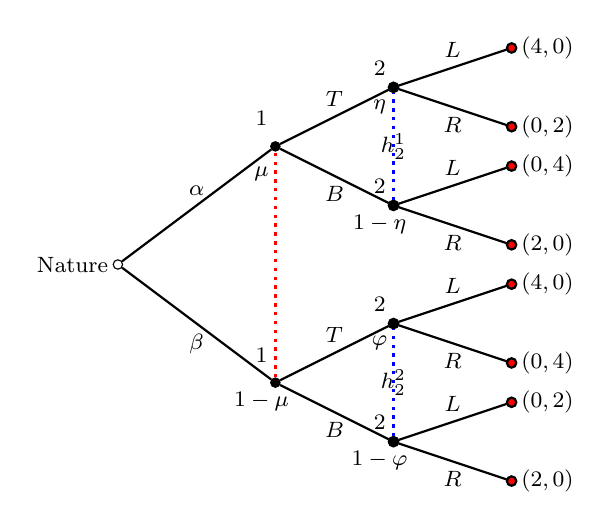
\begin{tikzpicture}
 		[
 		grow =right,
 		font=\footnotesize,
 		edge from parent/.style={draw,thick}
 		]
 		
 		% Two node styles: solid and hollow
 		\tikzstyle{solid node}=[circle,draw,inner sep=1.2,fill=black];
 		\tikzstyle{end node}=[circle,draw,inner sep=1.2,fill=red];
 		\tikzstyle{hollow node}=[circle,draw,inner sep=1.2];
 		
 		% Specify spacing for each level of the tree
 		\tikzstyle{level 1}=[level distance=20mm,sibling distance=30mm]
 		\tikzstyle{level 2}=[level distance=15mm,sibling distance=15mm]
 		\tikzstyle{level 3}=[level distance=15mm,sibling distance=10mm]
 		% The Tree
 		\node(0)[hollow node]{}
 		% \alpha
 		child{node[solid node]{} 
 			child{node[solid node]{}
	 			child{node[end node]{} edge from parent node[below]{$R$}}
	 			child{node[end node]{} edge from parent node[above]{$L$}}
 			edge from parent node[below]{$B$}}
	 		child{node[solid node]{}
	 			child{node[end node]{} edge from parent node[below]{$R$}}
	 			child{node[end node]{} edge from parent node[above]{$L$}}
 			edge from parent node[above]{$T$}}
		edge from parent node[below]{$\beta$}}
 		 		child{node[solid node]{} 
 			child{node[solid node]{}
 				child{node[end node]{} edge from parent node[below]{$R$}}
 				child{node[end node]{} edge from parent node[above]{$L$}}
 				edge from parent node[below]{$B$}}
 			child{node[solid node]{}
 				child{node[end node]{} edge from parent node[below]{$R$}}
 				child{node[end node]{} edge from parent node[above]{$L$}}
 				edge from parent node[above]{$T$}}
 			edge from parent node[above]{$\alpha$}}
 		;
 		% Information sets
		% of player 1
 		\draw[dotted, draw=red, very thick](0-1)to(0-2);
	 	% of player 2
		\foreach\x in {1, 2}\draw[dotted, draw=blue, very thick](0-\x-1)to(0-\x-2);
		\node at($(0-1-1)!.5!(0-1-2)$){$h_2^2$};
		\node at($(0-2-1)!.5!(0-2-2)$){$h_2^1$};
 		
 		% Players
 		% Nature
 		\node[left]at(0){Nature};
 		% player 1
 		\foreach \x in {1,2} \node[yshift=10, xshift=-5]at(0-\x){1};
		% player 2
		\foreach\x in {1,2} \foreach\y in {1,2} \node[yshift=7, xshift=-5]at(0-\x-\y){2};
		 		
 		% Specifying payoffs
 		\foreach\x in {1,2} \node[right]at(0-\x-2-2){$(4, 0)$};
 		\foreach\x in {1,2} \node[right]at(0-\x-1-1){$(2, 0)$};
 		\node[right]at(0-1-1-2){$(0, 2)$};
 		\node[right]at(0-2-2-1){$(0, 2)$};
 		\node[right]at(0-1-2-1){$(0, 4)$};
 		\node[right]at(0-2-1-2){$(0, 4)$};
 		
 		% Beliefs
 		\node[yshift=-7, xshift=-5]at(0-2-2){$\eta$};
 		\node[below, xshift=-5]at(0-2-1){$1 - \eta$};
 		\node[yshift=-7, xshift=-5]at(0-1-2){$\varphi$};
 		\node[below, xshift=-5]at(0-1-1){$1 - \varphi$};
 		\node[yshift=-10, xshift=-5]at(0-2){$\mu$};
 		\node[below, xshift=-5]at(0-1){$1 - \mu$};
 		
 		\end{tikzpicture}
 	\end{center}
 	%	\caption{A centipede game in extensive form}
 	%	\label{fig:ex1ext}
 \end{figure}

 Let the belief system of player 1 be described as $\mu = (\mu(\alpha), 1 - \mu(\alpha)$. Here, we are given that $\mu = (\frac{1}{2}, \frac{1}{2})$. Then, let the belief system of player 2 at the information set $h_2^1$ be $\eta = (\eta(T), 1 - \eta(T))$ and at the information set $h_2^2$ be $\varphi = (\varphi(T), 1 - \varphi(T))$.
 
 \begin{equation}
 	\begin{matrix}
	 	\text{Player 2 chooses }L\text{ at }h_2^1\text{ if}\\
	 	4(1 - \eta) > 2\eta\\
	 	1 - \eta > \frac{1}{2}\eta\\
	 	\frac{3}{2}\eta < 1 \\
	 	\eta < \frac{2}{3} \\
	 	\text{Player 2 chooses }L\text{ at }h_2^2\text{ if}\\
	 	2(1 - \varphi) > 4\varphi \\
	 	1 - \varphi > 2\varphi \\
	 	\varphi < \frac{1}{3}
 	\end{matrix} \qquad \begin{matrix}
	 	\text{Player 2 chooses }R\text{ at }h_2^1\text{ if}\\
	 	4(1 - \eta) < 2\eta\\
	 	1 - \eta < \frac{1}{2}\eta\\
	 	\frac{3}{2}\eta > 1 \\
	 	\eta > \frac{2}{3} \\
	 	\text{Player 2 chooses }R\text{ at }h_2^2\text{ if}\\
	 	2(1 - \varphi) < 4\varphi \\
	 	1 - \varphi < 2\varphi \\
	 	\varphi > \frac{1}{3}
 	\end{matrix} \nonumber
 \end{equation}
 
 Suppose that $\eta < \frac{2}{3}$ and $\varphi < \frac{1}{3}$. Then, player 2 chooses $L$ at both information sets. Then, by sequential rationality, player 1 chooses $T$ at his information set regardless of $\mu$. Given the strategy $\gamma = (T, (L, L))$, statistically consistent belief $\eta$ should be $\eta = \frac{1}{\frac{1}{2}} = 2$ \Lightning.
 
Suppose that $\eta < \frac{2}{3}$ and $\varphi > \frac{1}{3}$. Given such a belief system, player 2 chooses $L$ at $h_2^1$ and $R$ at $h_2^2$. Then, 
\begin{equation}
	\begin{split}
		\pi_1(T; \mu)& = 4\mu = 2 \\
		\pi_1(B; \mu)& = 2(1 - \mu) = 1 \nonumber
	\end{split}
\end{equation}
Given the belief system $\mu = (\frac{1}{2}, \frac{1}{2})$, by sequential rationality, player 1 chooses $T$. This again implies that statistically consistent beliefs of player 2 should satisfy $\eta = \frac{1}{\frac{1}{2}} = 2$ and $\varphi = \frac{1}{\frac{1}{2}} = 2$ \Lightning.

Suppose that $\eta > \frac{2}{3}$ and $\varphi < \frac{1}{3}$. Given such a belief system, player 2 chooses $R$ at $h_2^1$ and $L$ at $h_2^2$. Then, 
\begin{equation}
\begin{split}
\pi_1(T; \mu)& = 4(1 - \mu) = 2 \\
\pi_1(B; \mu)& = 2\mu = 1 \nonumber
\end{split}
\end{equation}
Given the belief system $\mu = (\frac{1}{2}, \frac{1}{2})$, by sequential rationality, player 1 again chooses $T$. This again implies that statistically consistent beliefs of player 2 should satisfy $\eta = \frac{1}{\frac{1}{2}} = 2$ and $\varphi = \frac{1}{\frac{1}{2}} = 2$ \Lightning.
 
Suppose that $\eta > \frac{2}{3}$ and $\varphi > \frac{1}{3}$. Given such a belief system, player 2 chooses $R$ at both information sets. Then, player 1 gets payoff 2 regardless of the type of player 2 if he/she chooses $B$, which is strictly better than 0 if he/she chooses $T$. Hence, by sequential rationality, player 1 chooses $B$. This implies that statistically consistent beliefs of player 2 should satisfy $\eta = \frac{0}{\frac{1}{2}} = 0$ and $\varphi = \frac{0}{\frac{1}{2}} = 0$, which contradicts sequential rationality of $(B, R)$.

Hence, the set of WPBE pure strategies is empty.

\end{document}
